\documentclass[a4paper,titlepage]{article}
\usepackage[]{mcode}
\usepackage{natbib}
\usepackage{graphicx}
\usepackage{hyperref}
\usepackage{amsthm}
\usepackage{amsmath}
\usepackage[margin=2cm]{geometry}

\begin{document}

\begin{titlepage}
	\newcommand{\HRule}{\rule{\linewidth}{0.5mm}}
	\center

	%------------------------------------------------
	%   Logo
	%------------------------------------------------

	
\includegraphics[width=0.2\textwidth]{Crest.jpg}\\[1cm]

	%------------------------------------------------
	%	Headings
	%------------------------------------------------

	\textsc{\LARGE University of Exeter}\\[1.5cm]

	\textsc{\Large College of Engineering, Mathematics and Physical Sciences}\\[0.5cm]

	\textsc{\large ECM3735 - Group 8}\\[0.5cm]

	%------------------------------------------------
	%	Title
	%------------------------------------------------

	\HRule\\[0.4cm]

	{\huge\bfseries Finding the optimal strategy for the dice game `Pig'}\\[0.4cm]

	\HRule\\[1.5cm]

	%------------------------------------------------
	%	Authors
	%------------------------------------------------

	\LARGE\textit{Authors}\\
	\begin{minipage}{0.4\textwidth}
		\begin{flushleft}
			\large
			S. \textsc{Bayliss}\\
			A. \textsc{Dunford}\\
			E. \textsc{Morison}\\
			J. \textsc{Peet}\\
			L. \textsc{Sutton}
		\end{flushleft}
	\end{minipage}
	~
	\begin{minipage}{0.4\textwidth}
		\begin{flushright}
			\large
			C. \textsc{Crawford}\\
			R. \textsc{Jones}\\
			C. \textsc{Nash}\\
			A. \textsc{Smith}
			\vspace*{10pt§}
		\end{flushright}
	\end{minipage}

	\vfill\vfill
	\textit{Supervisor}\\
	Dr. B. \textsc{Cooper}

	%------------------------------------------------
	%	Date
	%------------------------------------------------

	\vfill\vfill\vfill

	{\large\today}
	\vfill

	%------------------------------------------------
	%	Abstract
	%------------------------------------------------

	\newpage
	\begin{abstract}
	\textit{Insert abstract here}
	\end{abstract}
\end{titlepage}

	%------------------------------------------------
	%	Contents
	%------------------------------------------------

\tableofcontents
\newpage

\section{Introduction}
\subsection{Aims and Objectives}
josh
\subsection{History of Pig}
\subsubsection{Basics of Pig}
The dice game `pig' is played by 2 people rolling a die. The number on the die signifies the points gained on that roll, which are collated in a sum total of points for the turn. These points can be banked to bring a players turn to an end. However, the points in this rolling total can be lost if the player rolls a $1$, this will also automatically bring their turn to an end. The aim of the game is to be the first player to have a banked total of points greater than or equal to $100$.
\\
\\
The probabilities of winning the game from any position can be simplified down into sets of linear equations. Suppose I have 2 strategies A and B. Consider that it is A's turn and we are in position ($i,j,k$) where $i$ is A's banked points, $j$ is B's banked points, and $k$ is A's sum total of points so far on this turn. Let $P_{ijk}$ denote the probability of A winning from the current position and $Q_{ijk}$ denote probability of B winning from the equivalent position (where $i$ then represents B's banked points etc.). Then, \begin{equation}\label{1.2.1.a}
p_{ijk} = \dfrac{1}{6} (1-Q_{ij0}) + \dfrac{1}{6}\sum^{6}_{r=2}P_{ijk+r}
\end{equation}
 if A rolls and
 \begin{equation}\label{1.2.1.b}
 p_{ijk} = 1-Q_{jik}
 \end{equation}
 if A banks their points.
\subsubsection{Nellers Work}
In \textit{Dice Games Properly Explained}, Reiner Knizia takes the view of each roll of the die in `pig' as a bet of not rolling a $1$. He viewed the best strategy as ``Whenever your accumulated points are less than 20, you should continue throwing, because the odds are in your favour.''\cite{knizia2010dice}. However, Todd W Neller stated ``\textit{risking points is not the same as risking the probability of winning.}''\cite{neller2004optimal}, from this Neller proceeded to find a more optimal solution for `pig' by taking the maximum of equation \ref{1.2.1.a} and equation \ref{1.2.1.b}. This was not possible however as he ended up with an equation of the form $x=$max$ (A_1 x+b_1,A_2 x+b_2)$ for which there is no known general method. As a result Neller implemented value iteration to calculate an accurate estimate for the probabilities at each position $(i,j,k)$ for both bank and roll. Figure \ref{figure1} shows the resulting optimal strategy where you should roll if you are below the surface of the graph and bank if above.

\begin{figure}
\centering
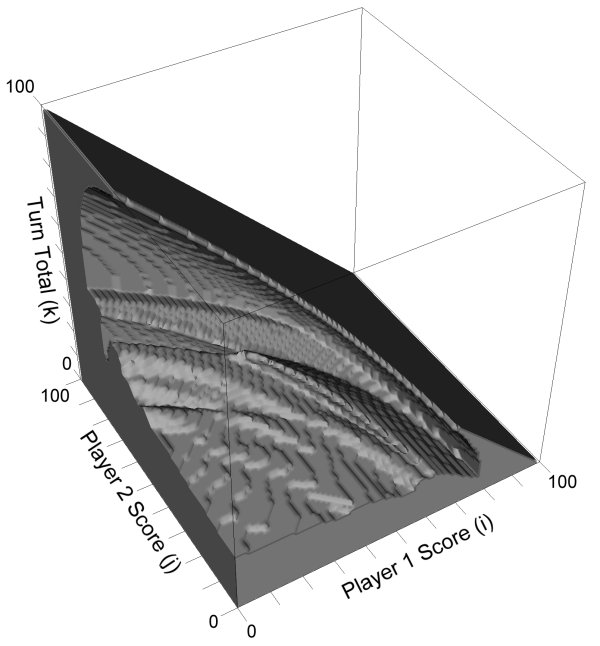
\includegraphics[width=0.5\textwidth]{neller_optimal_solution}
\caption{roll\slash hold boundary for the optimal Pig play policy (Neller)\label{figure1}}
\end{figure}
\begin{figure}
\centering
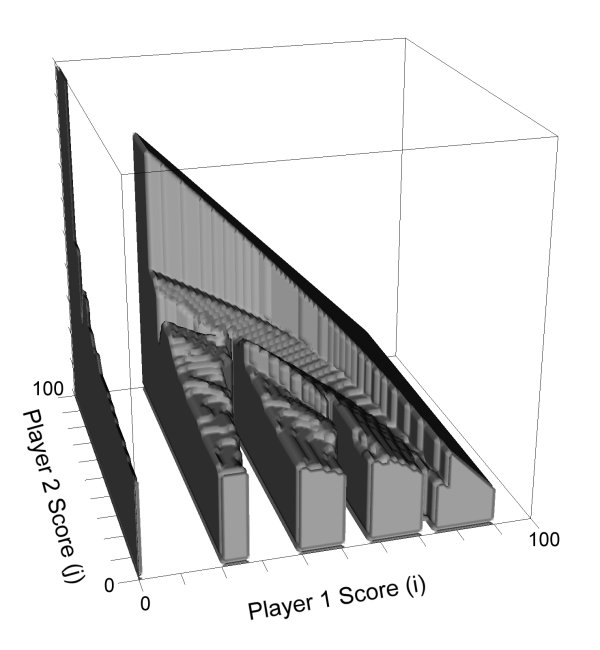
\includegraphics[width=0.5\textwidth]{neller_optimal_solution_2}
\caption{all of the states reachable by an optimal player (Neller)\label{figure2}}
\end{figure}

\subsection{Optimal Stratergy}
chris C
\subsection{Preliminary Findings}
chris N


\section{Methodology}
\subsection{Group Organisation}
Mia
\subsubsection{Meetings}
\subsubsection{Creation of Prject Plan}

\subsection{Piglet}
Chris C
\subsubsection{Hand Written notes}
\subsubsection{Coding Pig}
\subsubsection{Piglet Findings}

\subsection{Pig}
anthony and rhodri
\subsubsection{Expansion from Piglet}

I DID SOMETHING IOMPORTANT HERE

\subsubsection{Debugging of the code}
\subsection{Behavioural Economics}
Mia and Josh

\subsection{Statistical Testing}
eliot and sam
\subsubsection{Fair test}
\subsubsection{Theory of Hypothosis testing}
\subsubsection{Running of tests}


\section{Findings}
\subsection{Pig}
\subsubsection{Did we solve Pig}
{\tiny YES.}

\subsection{Behavioural Economics}
\subsubsection{Do players stick to their risk preference}
\subsubsection{Players Interactions}

\subsection{Statistical Testing}
\subsubsection{Non-transitivity}
\subsubsection{Testing against our optimal}
\subsubsection{Testing against Nellers optimal}


\section{Conclusions}
\subsection{Overall findings}
\subsection{Determination of human affects on the optimal stratergy}
\subsection{Comparison to Nellers stratergy}

\nocite{*}
\bibliographystyle{alpha}
\bibliography{Pig_bib}
\end{document}
